\chapter{The Generic Meta-Model Test Suite}
\label{chapter:metaModelTestSuite}

\begin{flushright}
\textit{Chapter written by Claas Wilke}
\end{flushright}

To test the adaptation of a meta-model to the pivot model of \acl{DOT4Eclipse}, the toolkit provides a generic test suite that can be simply instantiated by each adapted meta-model. This chapter shortly presents, how the generic meta-model test suite can be instantiated to test an adapted meta-model.



\section{The Test Suite Plug-in}

The generic meta-model test suite is located in the plug-in \code{tudresden.ocl20.pivot.meta\-mo\-dels.\linebreak[0]test}. The test suite provides a set of JUnit tests, that check the functionality of all operations that must be adapted by every meta-model that shall be adapted to the pivot model. The adaptation of a meta-model to the pivot model is explained in Chapter \ref{chapter:pivotModelAdaptation}. The test suite contains about 150 Junit tests.

To instantiate the generic test suite for a new adapted meta-model, only two resources must be provided: (1) a model modeled in the newly adapted meta-model that contains instances of all pivot model types that shall be tested, and (2) a Java class that instantiates the test suite with the modeled model. During test execution, the generic test suite uses the provided model to test the meta-model (see Figure \ref{pic:metaModelTestsuite:genericTestSuite}). Both, the model and the Java class are shortly presented in the following sections.

\begin{figure}[!t]
	\centering
		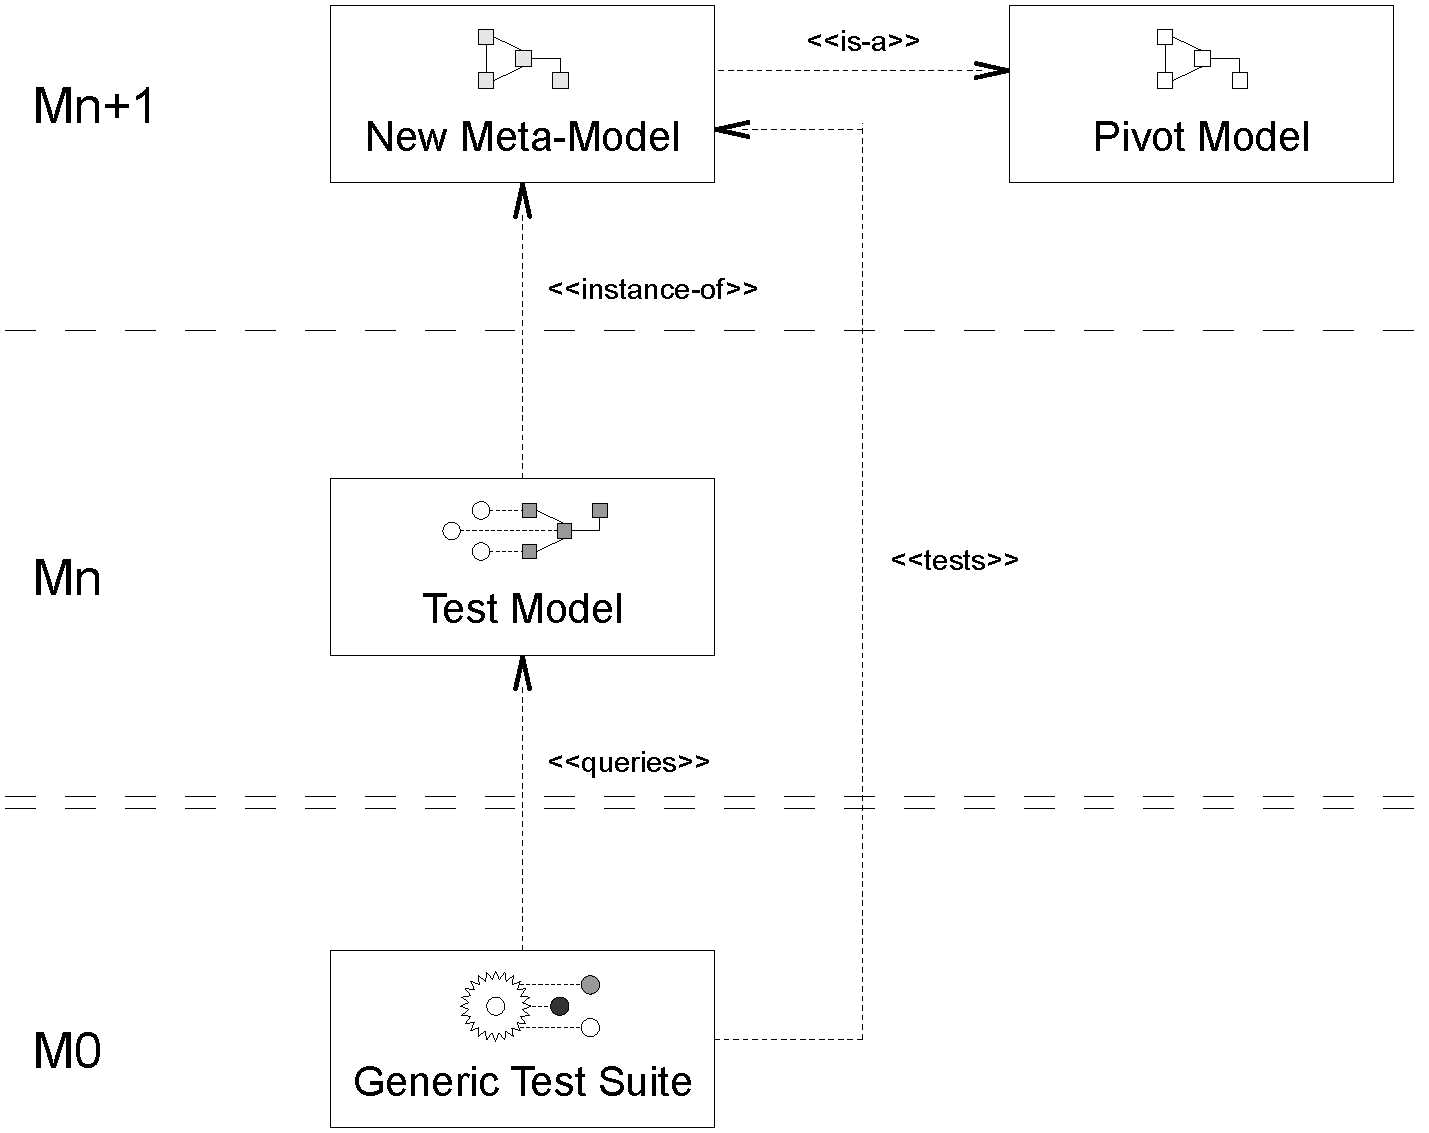
\includegraphics[width=0.80\textwidth]{figures/metamodeltestsuite/genericTestSuite.pdf}
	\label{pic:metaModelTestsuite:genericTestSuite}
	\caption{The Generic Meta-Model Test Suite in respect to the Generic Three Layer Ar\-chi\-tec\-ture}
\end{figure}



\section{The required Model to test a Meta-Model}

Figure \ref{pic:metaModelTestsuite:testModel} shows the test model that must be implemented in a meta-model that shall be tested with the generic meta-model test suite. At a first sight, the model seems to be very complex. But many of the contained features are optional, because some data structures and types of the pivot model could be (but do not have to be) implemented by a meta-model. E.g., a meta-model can provide a enumeration type but not has to. If a structure is not provided by a test model, the test suite will print a warning during test execution that the expected structure has not been found. If the structure is not adapted intentionally, the warnings can be ignored. In the following, all types and relations of the test model are explained shortly.

\begin{sidewaysfigure}[!p]
	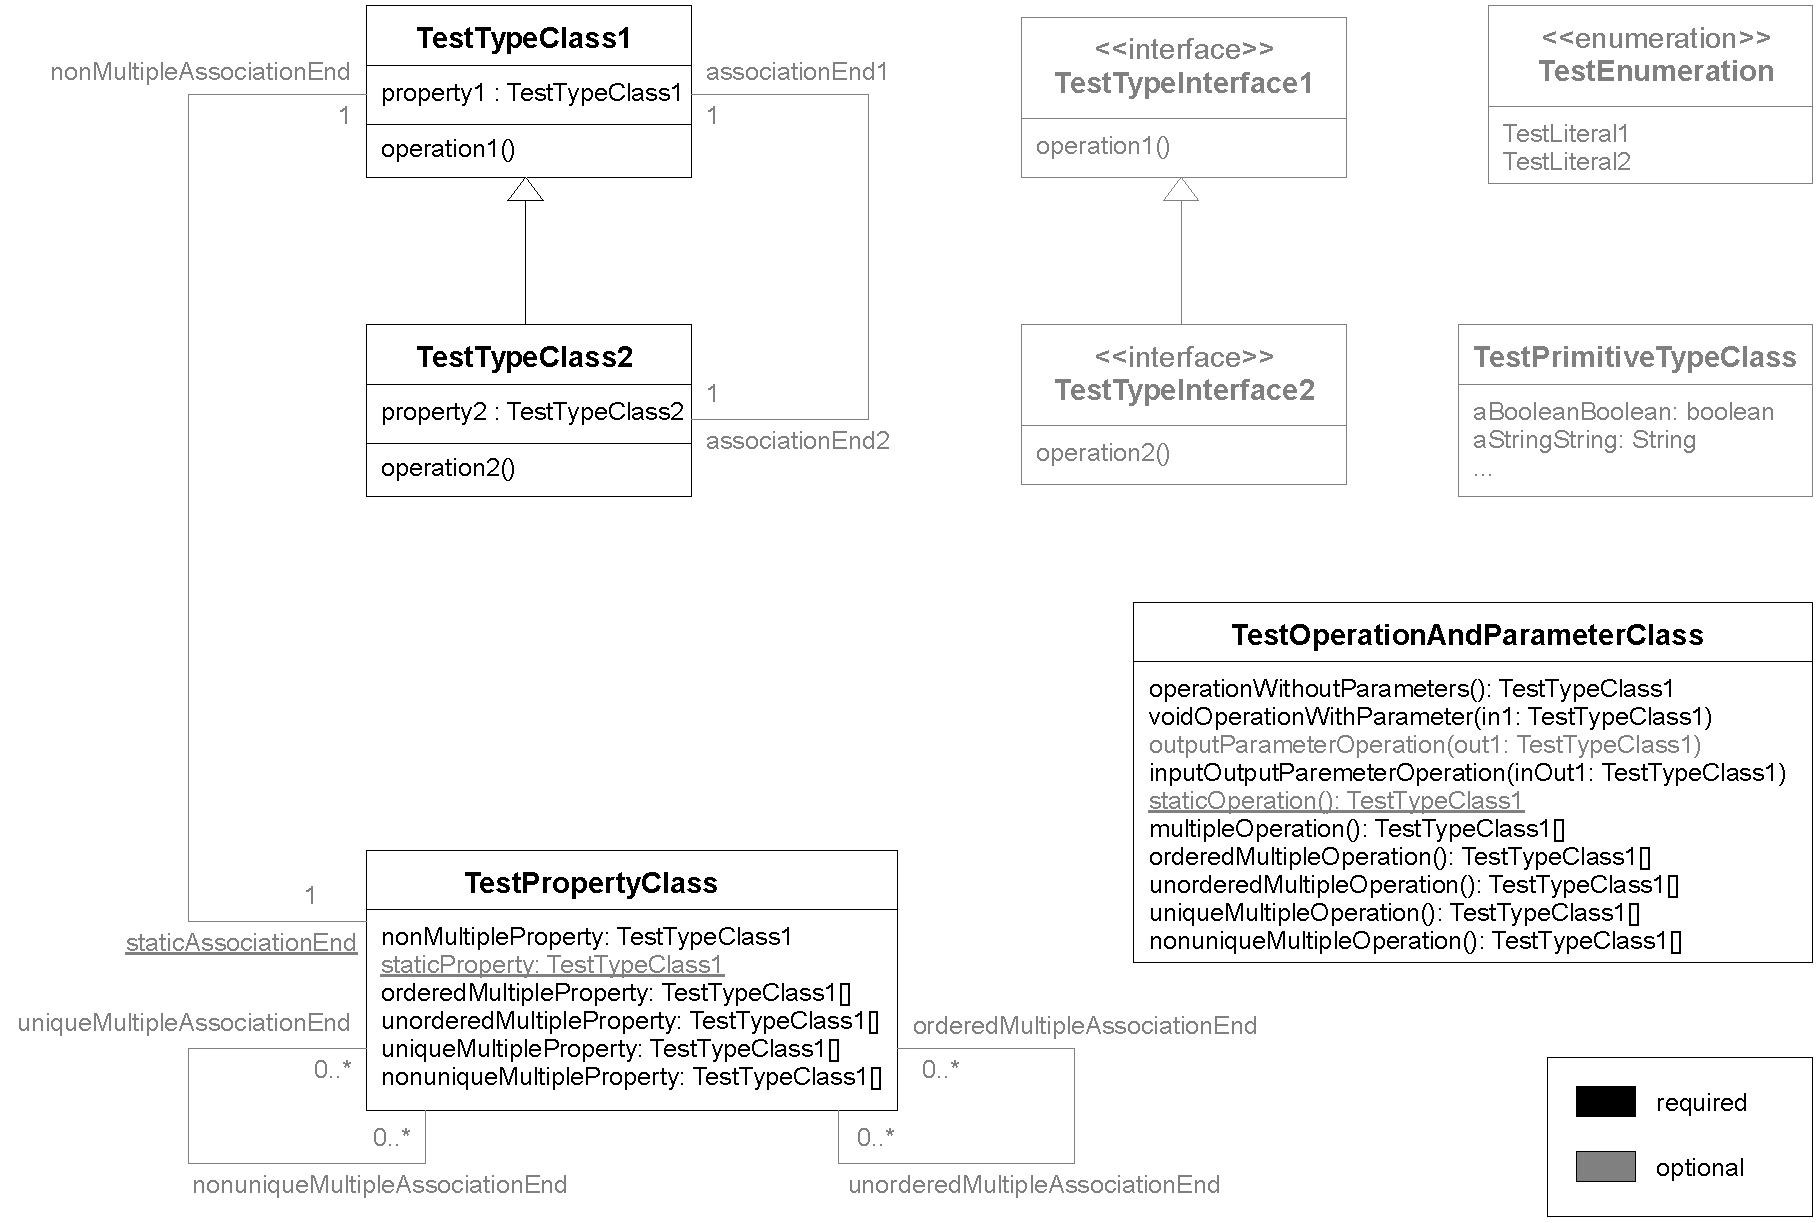
\includegraphics[width=0.85\textwidth]{figures/metamodeltestsuite/testModel.pdf}
	\caption{The required Test Model to test a Meta-Model's adaptation. The gray parts are optional.}
	\label{pic:metaModelTestsuite:testModel}
\end{sidewaysfigure}


\subsection{TestTypeClass1 and TestTypeClass2}

As their name already tells us, the classes \code{TestTypeClass1} and \code{TestTypeClass2} are used to test the adaptation of \code{Types}. Each meta-model has to provide types, thus, these classes are required. Both classes provide an operation and a property. The association between the two classes is optional because not all meta-models contain associations. But the generalization between \code{TestTypeClass2} and \code{TestTypeClass1} is required.


\subsection{TestTypeInterface1 and TestTypeInterface2}

Besides classes, some meta-models also provide a second type that must be mapped to the pivot model type \code{Type}, which is the interface type. To test the adaptation of the \code{Type} element for meta-models that have both, classes (or types) and interfaces, the test model contains two interfaces \code{TestTypeInterface1} and \code{TestTypeInterface2}. They are optional and can be used to test the adaptation of interfaces. E.g., a meta-model that adapts both classes and interfaces is the \acs{UML}2 meta-model located in the plug-in \code{tudresden.ocl20.pivot.metamodels.uml2}.


\subsection{TestEnumeration}

To test the adaptation of a \code{Enumeration} type, the class \code{TestEnumeration} can be used. Because enumerations are not part of every meta-model, this class of the test model is optional.


\subsection{TestPrimitiveTypeClass}

A special class in the test model is the class \code{TestPrimitiveTypeClass}. This class contains a property for each primitive type of the adapted meta-model that shall be tested. Each property has the type of the \code{PrimitiveType} whose adaptation shall be tested. Important is the name of the property. If the property's name starts with \code{aBoolean}, the type is tested as adapted to a pivot model's \code{PrimitiveType} of the kind \code{Boolean}. If the name starts with \code{anInteger} instead, the types is tested as an \code{Integer}. E.g., the example property \code{aStringString} shown in \code{TestPrimitiveTypeClass} in Figure \ref{pic:metaModelTestsuite:testModel} is tested as adapted to a \code{String}. Table \ref{tab:metaModelTestSuite:kindAdaptation} shows the adaptation of the different property name prefixes to the different \code{PrimitiveTypeKinds}.

\begin{table}[h]
		\begin{tabular}{|p{7cm}|p{7cm}|}
    \hline
    \textbf{Property Name Prefix} & \textbf{Expected PrimitiveTypeKind} \\
    \hline
    \code{aBoolean...} & \code{Boolean} \\			
    \hline
    \code{anInteger...} & \code{Integer} \\			
    \hline
    \code{aReal...} & \code{Real} \\			
    \hline
    \code{aString...} & \code{String} \\			
    \hline
		\end{tabular}
	\caption{The adaptation of properties' name prefixes to PrimitiveTypeKinds.}
	\label{tab:metaModelTestSuite:kindAdaptation}
\end{table}


\subsection{TestPropertyClass}

The class \code{TestPropertyClass} contains properties to test the right adaptation of the pivot model element \code{Property}. Additionally, the class has many associations that can be used to test the adaptation of a second property type for associations (like in the \acs{UML}2 meta-model, plug-in: \code{tudresden.ocl20.pivot.metamodels.uml2}). Thus, all associations are optional and are not required to test a meta-model's adaptation. The names of the contained properties are self-explainable: The property \code{nonMultipleProperty} is used to test the adaptation of a \code{Property} that cannot contain multiple values. The property \code{staticProperty} represents a static \code{Property} and is optional because not all meta-models contain a \code{static} modifier. The other properties are used to test multiple properties that are ordered, unordered, unique and non-unique.


\subsection{TestOperationAndParameterClass}

Similar to the class \code{TestPropertyClass} (presented above), the class \code{TestOperationAnd\-Pa\-ra\-me\-ter\-Class} contains operations to test the adaptation of all different kinds of \code{Operations}. Additionally, the class is also used to test the adaptation of \code{Parameters} of operations. Some of the operations are optional (like the static operation and the operation with an output value), others are required.


\section{Instantiating the Generic Test Suite}

As mentioned above, to initialize the generic meta-model test suite, only one Java class must be implemented that instantiates the test suite with the test model implemented in the adapted meta-model. Listing \ref{list:metaModelTestSuite:constraints01} shows a Java class that instantiates the test suite to test the \acs{UML}2 meta-model.

\lstset{
  language=Java
}
\begin{lstlisting}[caption={An instantiation of the generic meta-model test suite.}, captionpos=b, label=list:metaModelTestSuite:constraints01, float]
import tudresden.ocl20.pivot.metamodels.test.MetaModelTestPlugin;
import tudresden.ocl20.pivot.metamodels.test.MetaModelTestSuite;

@Suite.SuiteClasses(value = { MetaModelTestSuite.class })
public class TestUML2MetaModel extends MetaModelTestSuite {

  /** The id of the {@link IMetamodel} which shall be tested. */
  private static final String META_MODEL_ID = UML2MetamodelPlugin.ID;

  /** The path of the model which shall be tested. */
  private static final String TEST_MODEL_PATH = "model/testmodel.uml";

  /**
   * <p>
   * Prepares the {@link MetaModelTestSuite}.
   * </p>
   */
  @BeforeClass
  public static void setUp() {

    MetaModelTestPlugin.prepareTest(UML2MetaModelTestPlugin.PLUGIN_ID, 
      TEST_MODEL_PATH, META_MODEL_ID);
  }
}
\end{lstlisting}

Important is that the class provides a JUnit test suite (according to JUnit 4 conventions), that contains the \code{MetaModelTestSuite} (line 4). Additionally, the class only has to provide a \code{setUp()} method that can be used to setup the test suite before execution (lines 13 to 23). Inside the \code{setUp()} method, the operation \code{MetaModelTestPlugin.prepareTest(String, String, String)} must be invoked. The method initializes the environment of the generic test suite by setting three arguments:

\begin{enumerate}
	\item The \code{ID} of the plug-in that contains the test model used for testing (e.g., \code{tudresden.ocl20.\linebreak[0]pivot.\linebreak[0]metamodels.uml2.test},
	\item The location of the test model relative to the plug-in's root folder (e.g., \code{model/testmodel.\linebreak[0]uml}),
	\item And the \code{ID} of the meta-model that shall be tested (e.g. \code{tudresden.ocl20.pivot.meta\-mo\-dels.\linebreak[0]uml2}.
\end{enumerate}

Afterwards, the implemented Java class can be executed as a \eclipse{JUnit Plug-in Test} in Eclipse. The test suite should then inform you (by failed test cases) which parts of your meta-model adaptation are wrong implemented or missing. As mentioned above, warnings caused by missing parts of the test model--that were not implemented intentionally--can be ignored.


\section{Summary}

This chapter shortly introduced into the generic meta-model test suite of \acl{DOT4Eclipse}. For further details of the test suite investigate the test suite plug-in \code{tudresden.ocl20.pivot.\linebreak[0]metamodels.test} or the existing test suite instantiations in the plug-ins \code{tudresden.ocl20.pivot.\linebreak[0]metamodels.uml2.test}, \code{tudresden.ocl20.pivot.metamodels.ecore.test}, or \code{tudresden.\linebreak[0]ocl\-20.pivot.metamodels.java.test}.
